\section{Use-Case}
Der folgende Use-Case beschreibt eine Interaktion des Benutzers mit dem Frontend für das Anzeigen von Messdaten und das Einstellen von neuen Kontrollwerten, wie in Bild \ref{img:sequence} dargestellt.

\begin{figure}[h]
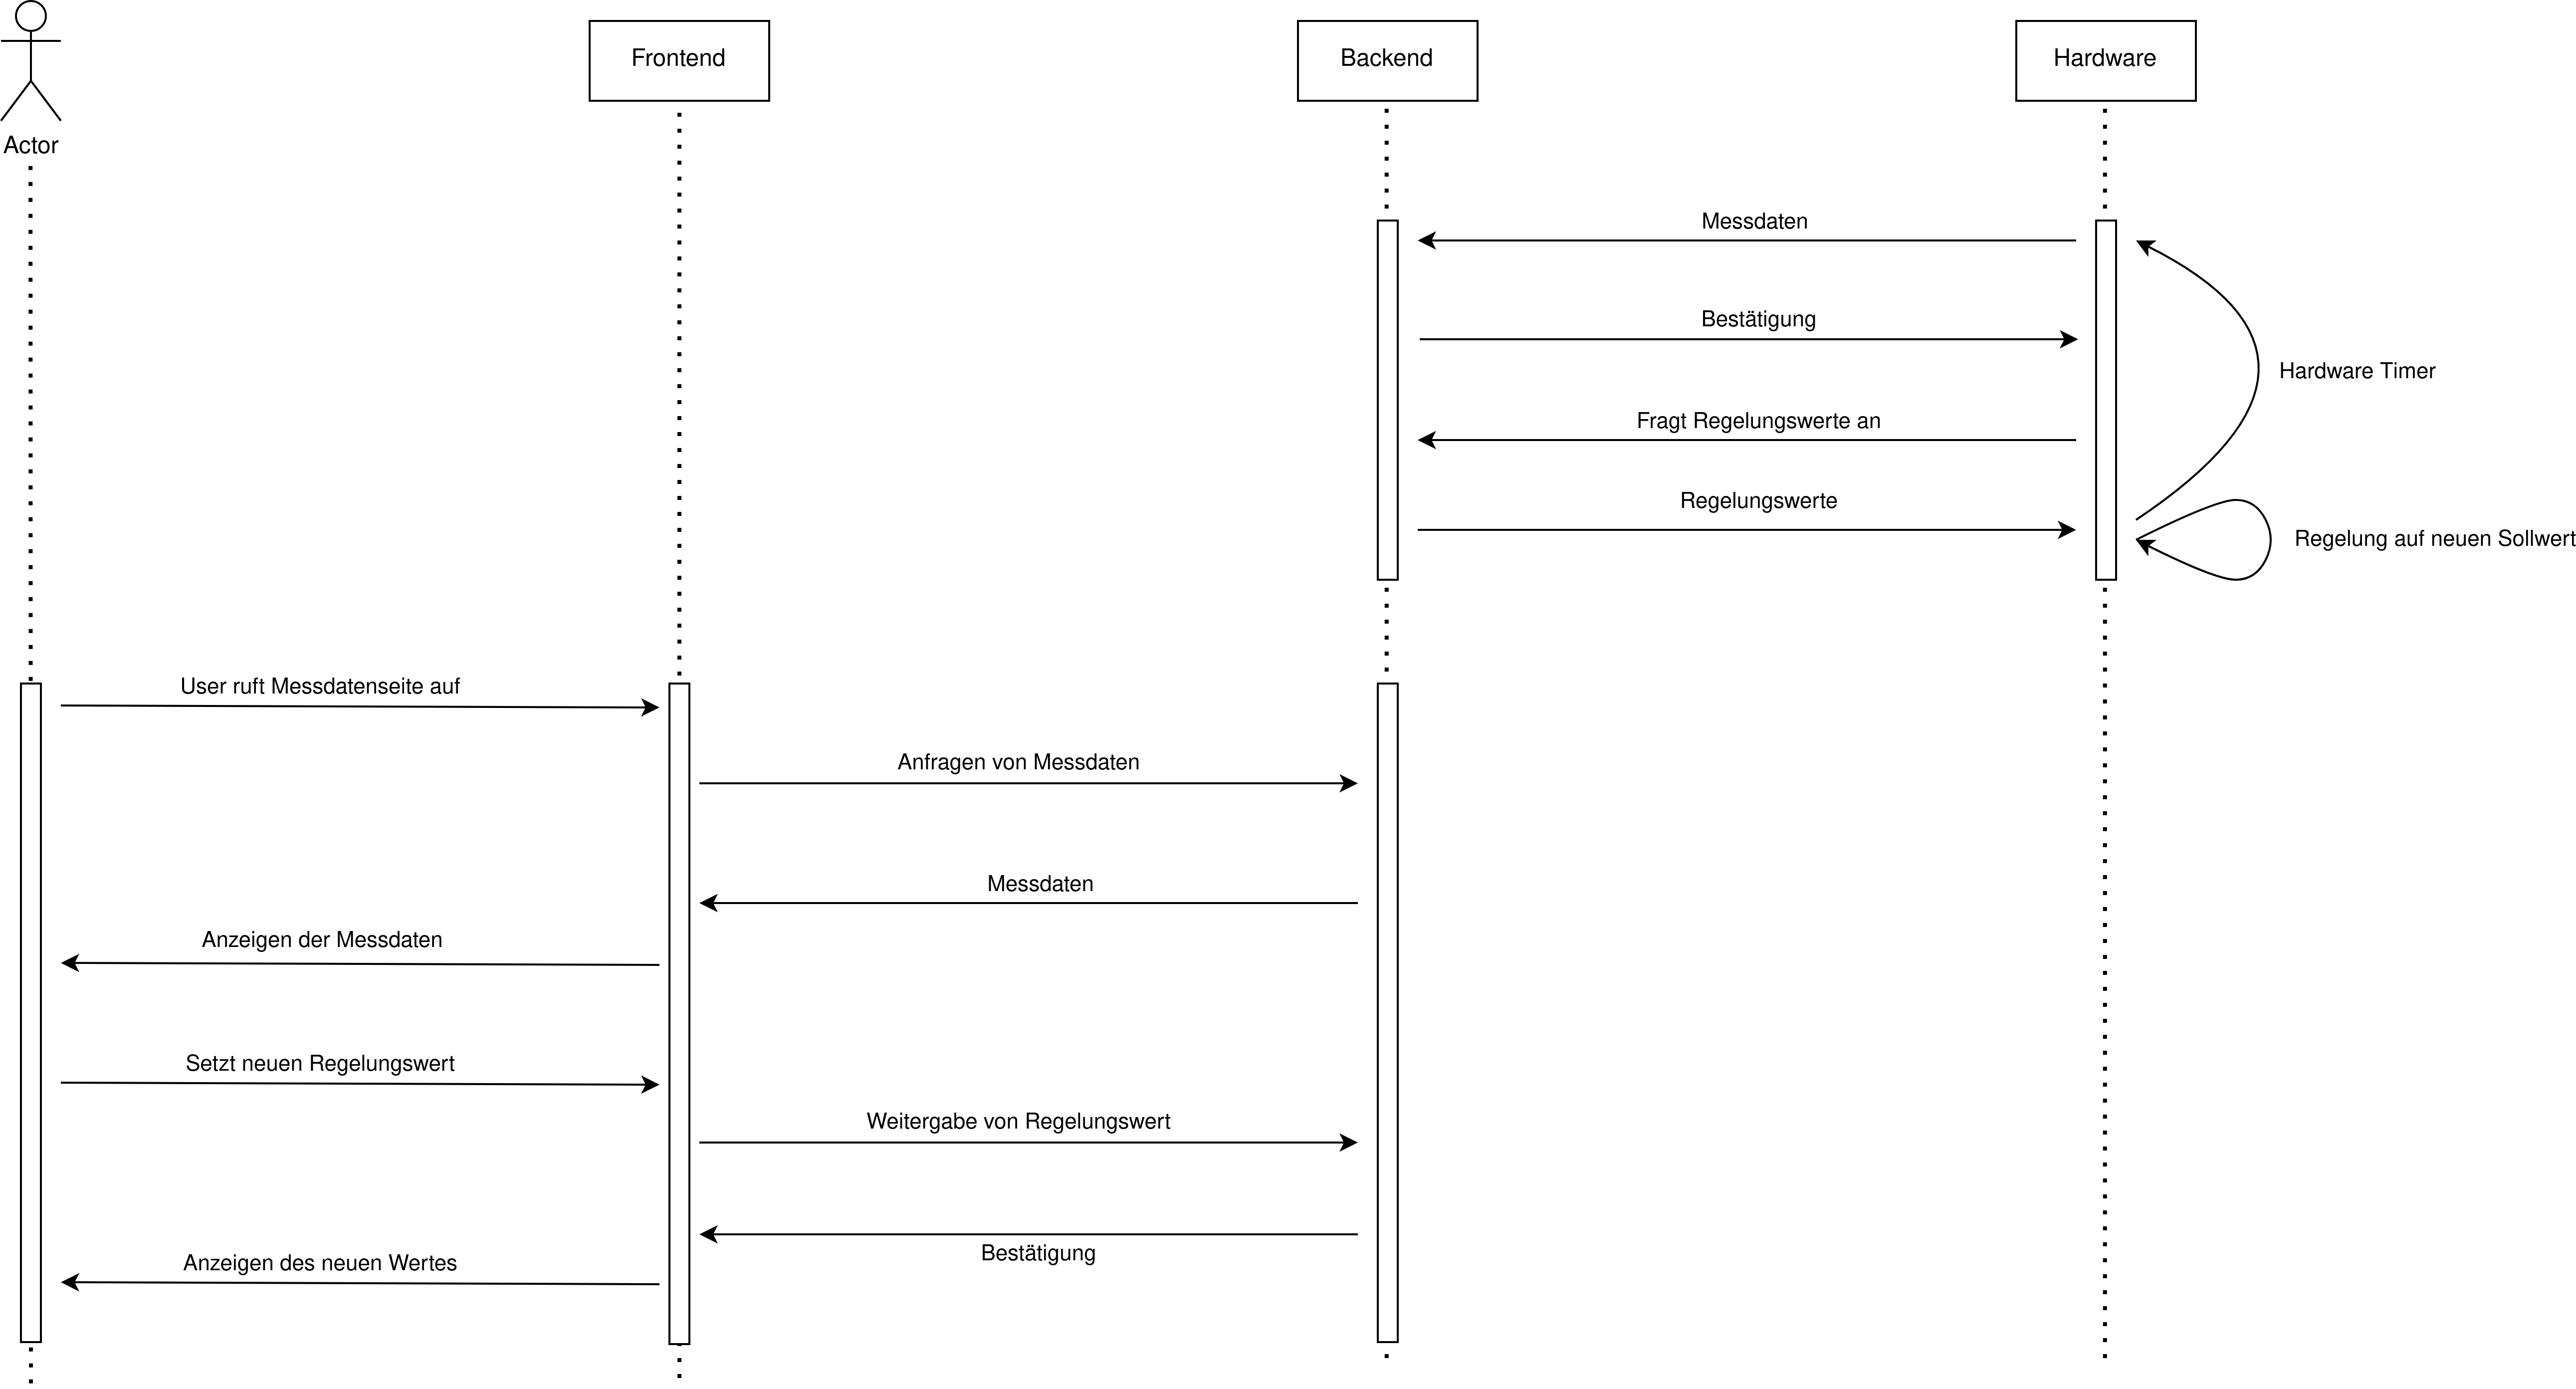
\includegraphics[width=\textwidth]{images/sequence_diagram.png}
\caption{Sequenzdiagramm einer Interaktion}
\label{img:sequence}
\end{figure}
%TODO: Insert numbers on sequence diagram transitions

In Bild \ref{img:sequence} kann besonders die Asynchronität der Interaktionen zwischen Frontend $\leftrightarrow$ Backend und Backend $\leftrightarrow$ Hardware gesehen werden.
Das Backend ist der Dreh- und Angelpunkt des ganzen Systems, woraus sich diese Beziehungen ergeben: die Hardware und das Frontend kennen das Backend, das Backend selbst macht jedoch keine Annahmen über über die anderen Systeme.
Von beiden Seiten wird also ein Pull-Ansatz verfolgt. \newline
Die Hardware kommuniziert mit dem Backend in periodischen Abständen.
Hierbei sendet die Hardware die neue Sensordaten an das Backend (1) und fragt die neusten Kontrollwerte für Aktoren ab (2).
Falls neue Kontrollwerte vorhanden sind, startet die Regelung der Aktoren zu diesem Kontrollwert hin.\newline
Die eben gesendeten Sensordaten werden vom Backend in einer Datenbank gespeichert, um sie dem Benutzer auf Abfrage anzuzeigen (3).
Sobald der Benutzer auf der Weboberfläche einen neuen Kontrollwert für einen Aktor einstellt, wird dieser vom Frontend an das Backend gesendet (4), um dort gespeichert, und auf Abruf an die Hardware weitergegeben zu werden

\pagebreak
